\documentclass[
marginals=nomargin
%fontsize=10pt, % Base font size
%twoside=false, % If true, use different layouts for even and odd pages (in particular, if twoside=true, the margin column will be always on the outside)
%secnumdepth=2, % How deep to number headings. Defaults to 2 (subsections)
%abstract=true, % Uncomment to print the title of the abstract
]{kaohandt}


% Choose the language
\usepackage[spanish]{babel} % Load characters and hyphenation
\usepackage[spanish=spanish]{csquotes}	% Spanish quotes

\usepackage{kaotheorems}
\usepackage{tikz}

% Load packages for testing
\usepackage{blindtext}
%\usepackage{showframe} % Uncomment to show boxes around the text area, margin, header and footer
%\usepackage{showlabels} % Uncomment to output the content of \label commands to the document where they are used

\graphicspath{{images/}{./}} % Paths where images are looked for

% Load mathematical packages for theorems and related environments.
\usepackage{kaotheorems}

% Load the bibliography package
\usepackage{kaobiblio}
\addbibresource{bibliography.bib} % Bibliography file

% Load the package for hyperreferences
\usepackage{kaorefs}


% Some shortcuts

% Real numbers, Natural numbers, etc.
\renewcommand{\P}{\mathbb{P}}
\newcommand{\E}{\mathbb{E}}
\newcommand{\R}{\mathbb{R}}
\newcommand{\Q}{\mathbb{Q}}
\newcommand{\Z}{\mathbb{Z}}
\newcommand{\C}{\mathbb{C}}
\newcommand{\N}{\mathbb{N}}

% Brackets
\newcommand{\qv}[1]{\langle #1 \rangle}

% (Conditional) expected value
\newcommand{\mean}[2][]{%
	\ifthenelse{\isempty{#1}}%
	{\mathbb{E}\!\left[#2\right]}%
	{\mathbb{E}\!\left[#2\,\middle|\,\mathcal{F}_{#1}\right]}%
}


%----------------------------------------------------------------------------------------

\begin{document}
	
	%----------------------------------------------------------------------------------------
	%	REPORT INFORMATION
	%----------------------------------------------------------------------------------------
	
	\title[]{Extendiendo la integral estocástica}
	
	\author[LM]{Lorenzo Martinelli\thanks{Universidad de Buenos Aires} }
	
	\date{\today}
	
	%----------------------------------------------------------------------------------------
	%	TITLE AND ABSTRACT
	%----------------------------------------------------------------------------------------
	
	\maketitle
	
	\margintoc
	
	\begin{abstract}
		La idea de esta monografía es dar un breve paseo sobre las propiedades básicas de los procesos de Levy, en particular, de los procesos de Poisson y Poisson compuesto con el fin de extender nuestra definición de integral estocástica a estos. Daremos además parte del marco teórico que permite extender la definición a un proceso de Lévy cualquiera.
	\end{abstract}
	
	%{\noindent\textbf{Keywords:} \LaTeX, Kao, handout, article, report}
	
	\medskip
	
	%----------------------------------------------------------------------------------------
	%	MAIN BODY
	%----------------------------------------------------------------------------------------
	
	\section{Introducción}
		Toda la teoría de integración estocástica que vimos durante el curso se apoyó principalmente en estudiar un tipo de proceso estocástico, el movimiento browniano, y que significa integrar respecto a este. Los supuestos que lo caracterizan son
		
		\begin{enumerate}
			\item incrementos independientes,
			\item incrementos estacionarios,
			\item trayectorias continuas.
		\end{enumerate}
			
		¿Qué ocurre si queremos ganar generalidad? Necesitamos eliminar, al menos, uno de estos. En este caso, vamos a olvidarnos de las trayectorias continuas para estudiar los llamados \emph{procesos de Lévy} con la intención de ampliar la definición de integral estocástica.
		
	\begin{marginfigure}[-4cm]
		\centering
		\includegraphics[width=\marginparwidth]{levy.jpg}
		\caption{Paul Pierre Lévy.}
	\end{marginfigure}
		
	
	\section{Procesos de Lévy}
	
	\marginnote[2cm]{	
		\begin{remark}
			Notemos que es posible reemplazar (L3) por $\lim_{t\to 0}{\P(|X(t)| > a)} = 0$ usando (L1) y (L2).
		\end{remark}
	}
	
	\begin{definition}[Proceso de Lévy]
		Un proceso estocástico $(X(t), t \geq 0)$ es un proceso de Lévy si cumple
		\begin{enumerate}[label=(L\arabic*)]
			\item $X(0) = 0$ casi seguramente,
			\item $(X(t), t\geq 0)$ tiene incrementos estacionarios e independientes,
			\item $(X(t), t\geq 0)$ es estocásticamente continua, es decir, para todo $a >0$, $s \geq 0$ se tiene que
			$$\lim_{t\to s}{\P(|X(t) - X(s)| > a)} = 0$$
		\end{enumerate}
	\end{definition}
	
	¿Qué proceso de Lévy ya conocemos? El movimiento browniano,\sidenote{Más aún, es el único con trayectorias continuas. No probaremos este resultado.} pero hay más, miremos un ejemplo que se deriva de este último.
	
	\begin{example}
		Sea $B(t)$ un movimiento browniano estándar y $T_s = \inf\{t: B(t) = s\}$, usando la propiedad fuerte de Markov uno puede ver que tiene incrementos independientes e identicamente distribuidos. Mientras que (L3) se hereda de la continuidad del movimiento browniano y, por lo tanto es un proceso de Lévy. Sin embargo, es posible ver que no tiene trayectorias continuas.
	\end{example}
	
	\subsection{Distribuciones infinitamente divisibles}
	
	Una noción que resulta importante estudiar es la de \emph{infinita divisibilidad}. Si bien prácticamente no la usaremos me parece importante mencionarla brevemente puesto que son fundamentales para ampliar la integral estocástica a procesos de Lévy, lo que sería una continuación directa de esta monografía.
	
	\begin{definition}
		Una variable aleatoria $X$ se dice que tiene una distribución infinitamente divisible si para cada $n \in \N$ podemos encontrar variables aleatorias i.i.d $Y_{1}^{(n)}, \dots, Y_{n}^{(n)}$ tales que
		$$X = Y_{1}^{(n)} + \dots + Y_{n}^{(n)}$$
	\end{definition}
	
	\begin{proposition}
		Si $(X(t), t\geq0)$ es un proceso de Lévy entonces $X(t)$ es infinitamente divisible para todo $t\ge0$.
	\end{proposition}
	
	\begin{proof}
		Basta considerar para cada $n\geq1$,
		$$Y_k^{(n)} = X(\frac{tk}{n}) - X(\frac{t(k-1)}{n})$$
		donde las $Y_k^{(n)}$ con $k = 1, 2, \dots, n$ son i.i.d por (L2). 
	\end{proof}
	
	\marginnote[-6cm]{
	\begin{example}
		Las variables aleatorias normales y poisson son infinitamente divisibles.
		\begin{itemize}
			\item Si $X \sim \mathcal{N}(m, \sigma^2)$ basta considerar $n$ variables aleatorias $\mathcal{N}(\frac{m}{n}, \frac{\sigma^2}{n})$. \\	
			\item Si $X \sim \mathcal{P}(\lambda)$ debemos considerar $n$ variables aleatorias poisson de intensidad $\frac{\lambda}{n}.$
		\end{itemize}
	\end{example}
	}
	
	\begin{marginfigure}[2cm]
		\centering
		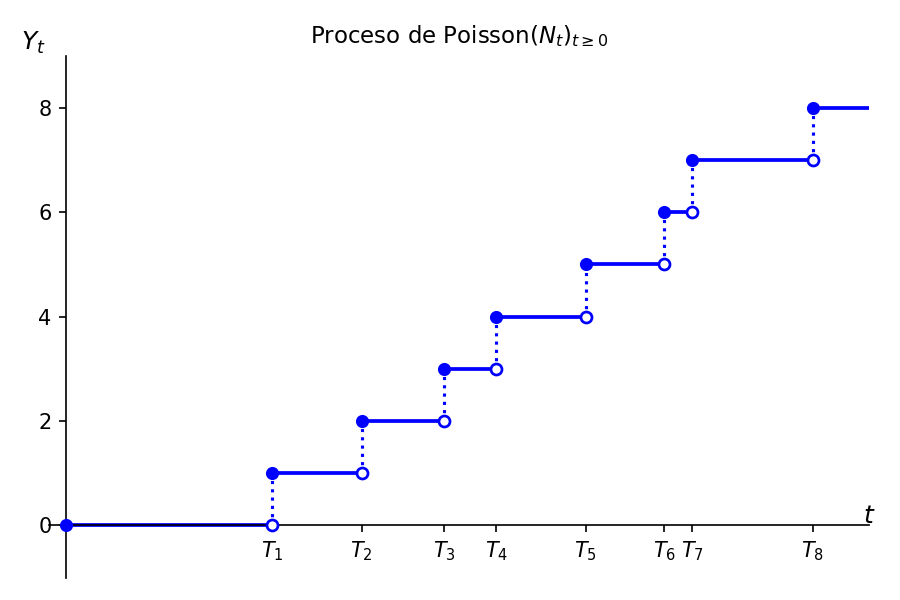
\includegraphics[width=\marginparwidth]{poisson.png}
		\caption{Trayectoria de un proceso de Poisson.}
	\end{marginfigure}
	
	\subsection{Proceso de Poisson}
	
	El \emph{proceso de Poisson} es un proceso de Lévy con saltos clásico que se obtiene al considerar saltos de tamaño uno a un ratio $\lambda$. Son procesos muy estudiados por sus aplicaciones en finanzas, biología, física entre otras.  
	
	\begin{definition}
		Un proceso de Poisson de intensidad $\lambda > 0$ es un proceso de Lévy $(N(t), t\geq 0)$ que toma valores en $\Z_{\geq 0}$ donde $N(t) \sim \mathcal{P}(\lambda)$, es decir,
		$$\P(N(t) = n) = \frac{(\lambda t)^{n}}{n!}e^{-\lambda t} $$
		para todo $n \in \Z_{\geq 0}.$
	\end{definition}
	
	Podemos definir también $(T_n, n \in \Z_{\geq 0})$, usualmente llamados tiempos de espera, como
	$$ T_n = \inf\{t\geq0: N(t) = n\}, \, T_0 = 0.$$
	Es posible ver que $T_n \sim \Gamma(n, \lambda)$ y los incrementos $T_n - T_{n-1}$ se distribuyen como exponenciales con esperanza $\frac{1}{\lambda}.$\sidenote{Si lo pensamos con cuidado tiene sentido que el tiempo que esperamos para dar un salto es el recíproco de la intensidad a la que ocurre.}
	
	\subsection{Poisson compuesto}
	
	Puede ser de nuestro interés que el tamaño del salto también sea aleatorio, de esta manera nacen los procesos de Poisson compuesto (CPP) que definimos más formalmente a continuación.
	
	\begin{definition}[CPP]
		Sea $(Z(n), n \in \N)$ una sucesión de variables aleatorias\sidenote{Notemos que si elegimos $Z(n)$ "trivialmente", es decir, tal que $\P(Z(n) = 1) = 1$ recuperamos el proceso de Poisson de antes.} i.i.d que toman valores en $\R^{d}$ con media $\mu$ y sea $(N(t), t\geq0)$ un proceso de Poisson con intensidad $\lambda$ independientes de los $Z(n)$, el CPP se define como 
		$$ Y(t) = Z(1) + \dots + Z(N(t)), \, \forall t\geq0.$$
	\end{definition}
	
	
	\begin{marginfigure}
		\centering
		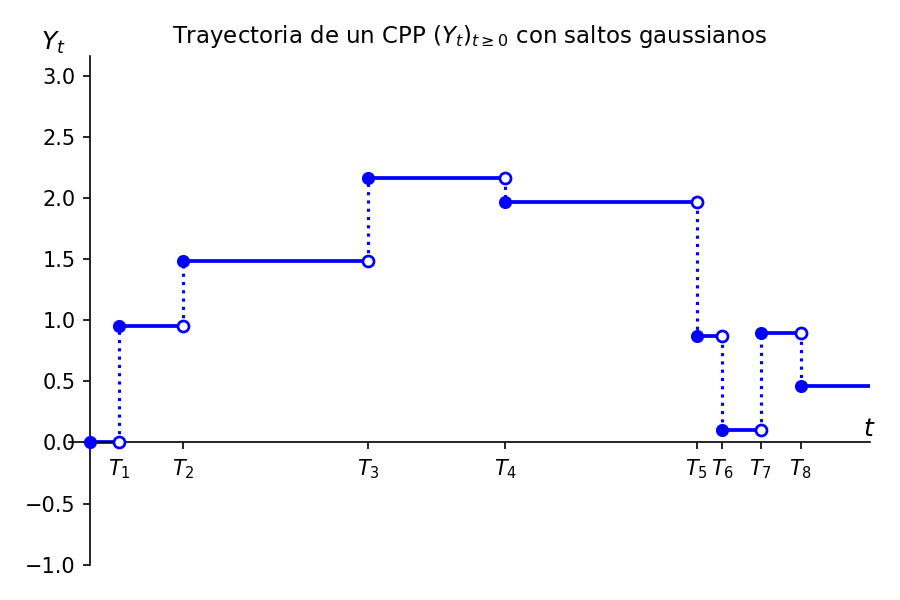
\includegraphics[width=\marginparwidth]{cpp_sample_path.png}
		\caption{CPP con $Z(K) \sim \mathcal{N}(0, 1)$.}
	\end{marginfigure}
	
	
	\begin{proposition}
		Un CPP es un proceso de Lévy.
	\end{proposition}
	
	\begin{proof}
		Basta chequear (L3), es decir, $\lim_{t\to0}{\P(|Y(t)|>a)} = 0.$ Condicionando y usando independencia tenemos que esta probabilidad es
		$$\sum_{n\geq0} \P(|\sum_{k=1}^{n} Z(k)| > a)\P(N(t) = n)$$
		notando que dado para $t < 1$ tenemos que $\frac{(\lambda t)^{n}}{n!}$ mayora a nuestra sucesión podemos meter el límite dentro de la sumatoria y tenemos el resultado. \sidenote{Hay que tener un poco de cuidado y mirar dos casos $n = 0$ y $n > 0$.}
	\end{proof}
	
	Para estudiar estas distribuciones infinitamente divisibles es útil considerar funciones características, y por simplicidad de la notación vamos a tomar logaritmo, para lo que hay que tener cierto cuidado pues toma valores en $\C.$
	
	\begin{marginfigure}
		\centering
		\includegraphics[width=\marginparwidth]{poisson_2.jpg}
		\caption{Siméon Denis Poisson.}
	\end{marginfigure}
	
	\begin{definition}[Exponente característico]
		Si $X$ es una variable aleatoria decimos que $\psi$ es su exponente característico si es una función continua que satisface 
		$$ \mean{e^{isX}} = e^{\psi(s)}, \, \psi(0) = 0.$$ 
	\end{definition} 
	
	
	\begin{definition}[Medida de Lévy]
		Sea $X(t) = \sum_{k=1}^{N(t)} Z(k)$ un proceso de Poisson compuesto, con $N(t)$ un proceso de Poisson de tasa $\lambda$ y $(Z(k))_{k\geq 1}$ i.i.d. con distribución $\mu^\#$, independientes de $N(t)$. Se define la \emph{medida de Lévy} de $X(t)$ como
		$$\mu(A) := \lambda\, \mu^\#(A), \qquad A \in \mathcal{B}(\mathbb{R}).$$
	\end{definition}
	
	Además, sin perdida de generalidad, asumimos que $\mu(\{0\}) = 0$ puesto que los saltos de altura cero no afectan al proceso.
	
	\marginnote[-2cm]{
	\begin{remark}
			Las medidas se definen de manera más general para cualquier proceso. En nuestro caso nos alcanza con esta.
	\end{remark}
	}
	
	\marginnote{
	\begin{remark}
		Para un proceso de Poisson usual, la medida de Lévy es una masa puntual, es decir $\mu(\{1\}) = \lambda$ y, $\mu(\R \setminus \{1\}) = 0.$ 
	\end{remark}
	}
	
	
	\begin{proposition}
		\labprop{cpp-caracteristica}
		Supongamos que $(X(t), t\geq 0)$ es un CPP con medida de Lévy $\mu$, con $X(0)=0$. Entonces
		$$\Psi(s) = \int_{-\infty}^{\infty} \big[e^{isx}-1\big]\, d\mu(x),$$
		$$Lf(x) = \int_{-\infty}^{\infty} \big[f(x+y)-f(x)\big]\, d\mu(y). $$
		Más aún, si
		$$\sigma^2 := \int x^2\, d\mu(x) < \infty, $$
		y
		$$m = \int x\, d\mu(x),$$
		entonces $M(t) = X(t) - tm$ es una martingala de cuadrado integrable con $\mathbb{V}[M(t)] = t\sigma^2$.
		\sidenote{No viene mal recordar la definición de $Lf(x)$, el generador de un proceso.
			\begin{definition}
				\labdef{generador}
				Sea $(X_t)_{t\geq0}$ un proceso de Markov. El \emph{generador} $L$ está dado por
				$$Lf(x) := \lim_{t\to0^+} \frac{\mean{f(X_t)\mid X_0=x} - f(x)}{t}$$
		\end{definition}}
	\end{proposition}
	
	\begin{proof}
		Sea 
		$$\phi(s) = \mean{e^{isY(j)}} = \int_{\R} e^{isx} d\mu^{\#}(x),$$
		la función característica de una variable aleatoria $Y(j)$. Miremos ahora, la característica de un CPP,
		$$\mean{e^{isX(t)}} = \sum_{n=0}^{\infty} \P(N(t) = n)\mean{e^{isX(t)} \, \middle| \, N(t) = n},$$
		dado que $N(t) = n$ tenemos que $X(t)$ se distribuye como $Y(1) + \dots + Y(n)$ y, en consecuencia, $\mean{e^{isX(t)} \, \middle| \, N(t) = n} = \phi(s)^n.$ Luego,
		\[
		\begin{aligned}
			\mean{e^{isX(t)}} &= \sum_{n=0}^{\infty} \frac{(\lambda t \phi(s))^{n}}{n!} e^{-\lambda t} \\
							  &= \exp{t \lambda(\phi(s) - 1)} \\
							  &= \exp{t \lambda(\int_{\R} [e^{isx} - 1] d\mu^{\#}(x))} \\
							  &= \exp{t \int_{\R} [e^{isx} - 1] d\mu(x))} 
		\end{aligned} 
		\]
		notemos que podemos meter el $1$ dentro de la integral pues $\mu^{\#}(\R) = 1.$  Ahora tenemos que mirar el generador del proceso, la idea central acá es que en un intervalo de tiempo muy chiquito o hay un solo salto o no hay ninguno con un error que viene dado por la probabilidad de que haya al menos dos, es decir,
		$$ \P(N(t) = 0) = 0) = 1 - \lambda t + o(t) \quad  \P(N(t) = 0) = 1) = \lambda t + o(t),$$
		de esta manera,
		$$ \E[f(X(t)) | X(0) = x] = (1 - \lambda t)f(x) + \lambda t \int_{\R} f(x + y) d\mu(y) + o(t),$$
		reorganizando,
		$$ \E[f(X(t)) | X(0) = x] - f(x) = t \int_{\R} [f(x + y) - f(x)] d\mu(y) + o(t),$$
		dividiendo por $t$ y tomando límite $t \to 0^{+}$ tenemos el resultado.
		Suponiendo que los momentos existen. Para cualquier entero positivo $n$, si
		$$\int_{-\infty}^{\infty} |x|^n\, d\mu(x) < \infty,$$
		entonces podemos diferenciar bajo el signo integral $n$ veces para ver que
		$$\Psi^{(n)}(s) = i^n \int_{-\infty}^{\infty} x^n\, e^{isx}\, d\mu(x).$$
		En particular,
		$$\Psi'(0) = i\int_{-\infty}^{\infty} x\, d\mu(x), \qquad \Psi''(0) = -\int_{-\infty}^{\infty} x^2\, d\mu(x),$$
		y como $\phi_{X(t)}(s) = \exp\{t\Psi(s)\}$ y $\Psi(0)=0$, obtenemos
		$$\phi'_{X(t)}(0) = t\Psi'(0) = it\int_{-\infty}^{\infty} x\, d\mu(x) = itm,$$
		$$\phi''_{X(t)}(0) = t\Psi''(0) + [t\Psi'(0)]^2 = -[t\sigma^2 + (tm)^2].$$
		Por lo tanto,
		$$\E[X(t)] = tm, \qquad \mathbb{V}[X(t)] = t\sigma^2.$$
		Si $\mathcal{F}_s$ denota la información contenida en $\{X(r) : r\leq s\}$ y $s<t$, entonces $X(t) - X_s$ es independiente de $\mathcal{F}_s$ y
		$$\mean[s]{X(t)} = X(s) + \mean[s]{X(t) - X(s)} = X(s) + \E[X(t) - X(s)] = X(s) + (t-s)m,$$
		y por lo tanto
		$$\mean[s]{X(t) - tm} = X(s) - sm.$$
		Esto muestra que $M_t$ es una martingala, y
		$$\E[M(t)^2] = \E[(X(t)-tm)^2] = \mathbb{V}[X(t)] = t\sigma^2.$$
	\end{proof}	
	
	\subsection{Proceso de Poisson compuesto compensado}
	
	Llamamos a $M(t) = X(t) - mt$ proceso de Poisson compuesto compensado (CCPP) asociado a $X(t).$ Es un proceso de Lévy. Si $L$ denota el generador de $X(t)$ entonces $M(t)$ tiene generador 
	$$L_{M}f(x) = Lf(x) - mf^{'}(x).$$
	Por otro lado, la variación cuadrática se define como para el movimiento browniano y tenemos
	$$\qv{X}_t = \lim_{n\to \infty} \sum_{j \leq tn}{[X(\frac{j}{n}) - X(\frac{j-1}{n})]}^{2}$$
	cómo todos los terminos son cero a menos que haya un salto tenemos que
	$$\qv{X}_t = \sum_{s \leq tn}{[X(s) - X(s-)]^2}.$$	
	A diferencia del movimiento browniano para un tiempo fijo no es constante. De manera similar obtenemos que $\qv{X}_t = \qv{M}_t.$
	
	A continuación, vamos a ver una proposición que generaliza el último resultado que vimos y que además da cierta intuición acerca del generador $L$.\sidenote{
	En algún sentido vamos a ver un análogo a la fórmula de Itô para CPP, recordemos que si $X(t)$ satisface 
	$$dX_t = m(X_t)dt + \sigma(X_t)dB_t,$$
	luego, 
	$$Lf(x) = m(x)f'(x) + \frac{\sigma^{2}(x)}{2}f^{''}(x).$$
	Por otro lado, Itô nos dice que 
	$$df(X_t) = Lf(X_t)dt + f^{'}(X_t)\sigma(X_t)dB_t.$$
	Es decir, que si 
	$$M_t = f(X_t) - \int_{0}^{t} Lf(X_s)ds $$
	es una martingala (local) que cumple que
	$$dM_t = f^{'}(X_t)\sigma(X_t)dB_S.$$
	}
		
	\begin{proposition}
		Supongamos que $X(t)$ es un CPP con medida de Lévy $\mu$, y supongamos que $f$ es una función continua tal que 
		$$\mean{f(X_t)^2 \, \middle | \, X_0 = x} < \infty \quad \forall x, t $$
		entonces,
		$$ M(t) = f(X_t) - \int_{0}^{t} Lf(X_s)ds$$
		es una martingala cuadrado integrable con 
		$$\qv{M}_t = \qv{f(X)}_t = \sum_{s\leq t} [f(X_s) - f(X_{s-})]^2.$$
	\end{proposition}

	\begin{proof}
		Comencemos probando que $M_t = M(t)$ es una martingala, es decir, que $\mean[s]{M_t} = M_s$ para $s < t.$ El argumento es esencialmente el mismo para todo $s$, por lo que vamos a suponer que $s = 0$ y que $X_0 = x.$ Tenemos que ver que 
		$$\mean{f(X_t) - f(X_0) - \int_{0}^{t} Lf(X_s)ds} = 0.$$
		Además, esto es igual para todo $t$ por lo que vamos a asumir $t=1.$ De esta manera,
		\[
		\begin{aligned}
			f(X_t) - f(X_0) - \int_{0}^{t} Lf(X_s)ds = \\
			\sum_{j=1}^{n}{f(X(\frac{j}{n})) - f(X(\frac{j-1}{n})) - \int_{\frac{j-1}{n}}^{\frac{j}{n}} Lf(X_s)ds}
		\end{aligned}
		\]
		y podemos escribir la esperanza de esta expresión como suma de otras dos expresiones
		\begin{equation}
			\sum_{j=1}^{n} \mathbb{E}\left[ f\left(X\left(\tfrac{j}{n}\right)\right) - f\left(X\left(\tfrac{j-1}{n}\right)\right) - \frac{1}{n} Lf\left(X\left(\tfrac{j-1}{n}\right)\right) \right],
			\tag{1}
		\end{equation}
		
		\begin{equation}
			\sum_{j=1}^{n} \mathbb{E}\left[ \frac{1}{n} Lf\left(X\left(\tfrac{j-1}{n}\right)\right) - \int_{(j-1)/n}^{j/n} Lf(X(s))\, ds \right].
			\tag{2}
		\end{equation}
		Por otro lado, recordemos que la definición de $Lf$ implica que
		$$\mean[t]{f(X_{t + \delta})} = f(X_t) + Lf(X_t)\delta + o(\delta),$$
		y en consecuencia
		$$\mean[t]{f(X_{t + \delta}) - f(X_t) - Lf(X_t)\delta } = o(\delta).$$
		Esto muestra que $(1)$ tiene n términos $o(1/n)$ y por lo tanto el límite es cero. Por otro lado, los terminos dentro de $(2)$ son cero a menos que ocurra un salto entre $\frac{j-1}{n}$ y $\frac{j}{n}.$ Esto ocurre con probabilidad $O(1/n)$ y, en ese caso el valor de la variable aleatoria es $O(1/n)$. Luego, la esperanza es $O(1/n^2)$ y el límite es 0. La cuenta de la variación cuadrática es esencialmente expandir el cuadrado y notar que todos los terminos se van a cero y sobrevive la variación cuadrática de $f(X_t).$
	\end{proof}
	
	\section{Integrando con respecto a un CPP}
	
	En esta sección daremos una definición (al fin) de qué significa integrar con respecto a un proceso de Poisson compuesto.
	
	Antes de comenzar, vamos a recordar brevemente qué es una función cadlag. Para un CPP las trayectorias $t \mapsto X_t$ son constantes a trozos y discontinuas en los saltos. Al igual que para el proceso de Poisson usual, hemos definido la trayectoria de modo que sea continua a derecha y tenga límites por izquierda. Llamamos \emph{càdlàg} a una función (también escrito \emph{cadlag}), abreviatura de \emph{continue à droite, limite à gauche}, si sus trayectorias son continuas a derecha en todo punto y tienen límites por izquierda. Es decir, para todo $t$, los límites
	\[
	X_{t+} = \lim_{s \downarrow t} X_s, \qquad X_{t-} = \lim_{s \uparrow t} X_s,
	\]
	existen y $X_t = X_{t+}$. Las trayectorias de un CPP son càdlàg. Podemos escribir
	\[
	X_t = X_0 + \sum_{0 \leq s \leq t} \big[X_s - X_{s-}\big].
	\]
	Aunque tal como está escrita esta suma es sobre una cantidad no numerable de tiempos $s$, el término $X_s - X_{s-}$ es no nulo únicamente en aquellos $s$ en los que la trayectoria es discontinua, y este es un conjunto finito.
	
	Ahora, sí definamos que significa integrar respecto a un CPP. La definición más natural posible, dado otro proceso $A_t$ es 
	$$\int_{0}^{t} A_s dX_s = \sum_{0\leq s\leq t} A_s [X_s - X_{s-}].$$ 
	Por el comentario que hicimos antes, esta suma está bien definida. Sin embargo, si queremos que cumpla buenas propiedades como la de Itô necesitamos pedir ciertas hipótesis.		
	
	Supongamos que $\mathbb{E}[X_1] = m$, $\mathrm{Var}[X_1] = \sigma^2$, y sea $M_t$ la martingala de cuadrado integrable $M_t = X_t - mt$. Entonces, si las trayectorias de $A_t$ son Riemann integrables, y la integral
	\[
	Z_t = \int_0^t A_s\, dM_s = \int_0^t A_s\, dX_s - m\int_0^t A_s\, ds
	\]
	está bien definida. Sea $\mathcal{F}_t$ la información contenida en $\{M_s : s \leq t\}$, que es la misma información contenida en $\{X_s : s \leq t\}$. En analogía con la integral de Itô, podríamos esperar que si $A_t$ es de cuadrado integrable, continua a trozos, y adaptada a $\{\mathcal{F}_t\}$, entonces $Z_t$ sería una martingala. Sin embargo, esto no siempre es así, como veremos a continuación.

	\begin{example}
		Supongamos que $X_t$ es el CPP que tiene saltos de tasa $1$ y, cuando salta, elige $\pm 1$ con la misma probabilidad. Es decir, la medida de Lévy de $X$ es la medida de probabilidad con $\mu(\{1\}) = \mu(\{-1\}) = 1/2$. Entonces $m=0$, $\sigma^2=1$, y $A_t = X_t - X_{t-}$ está adaptado a $\{\mathcal{F}_t\}$. Es discontinua únicamente en los saltos de $X_t$ y por lo tanto es continua a trozos. Sin embargo, si definimos la integral como antes, entonces
		\[
		\int_0^t A_s\, dX_s = \sum_{0 \leq s \leq t} \big[X_s - X_{s-}\big]^2,
		\]
		lo cual tiene esperanza positiva (ya que es no negativa y tiene probabilidad positiva de ser estrictamente positiva).
		
		¿Cuál es el problema? Estamos permitiendo una estrategia de apuesta que ve un salto en el instante $s$ e inmediatamente cambia la apuesta para aprovecharlo. En nuestro marco de trabajo, no vamos a permitir estos cambios instantáneos, restringiéndonos a estrategias que sean continuas a izquierda.	
	\end{example}
	
	\begin{proposition}
		Supongamos que $X_t$ es un CPP con $\sigma^2 < \infty$ y $M_t = X_t - mt$. Supongamos además que $A_t$ es un proceso que satisface:
		
		\begin{itemize}
			\item \textit{cada $A_t$ es medible respecto de $\{X_s : 0 \leq s \leq t\}$,}
			\item \textit{con probabilidad uno, las trayectorias de $A_t$ son continuas a izquierda, es decir, $A_t = A_{t-}$,}
			\item \textit{para todo $t < \infty$,}
			\[
			\int_0^t \mathbb{E}[A_s^2]\, ds < \infty.
			\]
		\end{itemize}
		
		\textit{Entonces}
		\[
		Z_t = \int_0^t A_s\, dM_s
		\]
		\textit{es una martingala de cuadrado integrable con}
		\begin{equation}
			\mathbb{E}\big[Z_t^2\big] = \sigma^2 \int_0^t \mathbb{E}[A_s^2]\, ds.
			\label{eq:1}
		\end{equation}
		
		En lugar de suponer que $A_s$ es continua a izquierda, podemos suponer que $A_s$ tiene trayectorias càdlàg, pero entonces cambiemos la definición que dimos antes por
		\[
		\int_0^t A_s\, dX_s = \sum_{0 \leq s \leq t} A_{s-} \big[X_s - X_{s-}\big].
		\]
	\end{proposition}
	
	\begin{proof}
		Si $s < t$, entonces como antes,
		\begin{equation}
			\mathbb{E}[A_s(M_t - M_s) \mid \mathcal{F}_s] = A_s\, \mathbb{E}[M_t - M_s \mid \mathcal{F}_s] = 0,
			\label{eq:6.11}
		\end{equation}
		\begin{align}
			\mathbb{E}[A_s^2(M_t-M_s)^2] &= \mathbb{E}\big[\mathbb{E}(A_s^2(M_t-M_s)^2 \mid \mathcal{F}_s)\big] \notag \\
			&= \mathbb{E}\big[A_s^2\, \mathbb{E}[(M_t-M_s)^2]\big] \notag \\
			&= \sigma^2 (t-s)\, \mathbb{E}[A_s^2]. \label{eq:6.12}
		\end{align}
		
		Para cada $t$, la probabilidad de que $M_{t-} \neq M_t$ es $0$. Por lo tanto, con probabilidad uno, para todo tiempo racional $t$, $M_t = M_{t-}$. Supongamos que $A_s$ es un proceso simple que cambia de valor únicamente en tiempos de la forma $\{0, 1/n, 2/n, 3/n, \ldots\}$. Entonces, con probabilidad uno, para todo $t$, si $j/n \leq t < (j+1)/n$,
		\[
		Z_t = \int_0^t A_s\, dM_s = \sum_{i=0}^{j-1} A\left(\frac{i}{n}\right)\left[M\left(\frac{i+1}{n}\right) - M\left(\frac{i}{n}\right)\right].
		\]
		Esta expresión usa el hecho de que $M_t = M_{t-}$ para todo tiempo racional $t$. Usando esta expresión y \eqref{eq:6.11} y \eqref{eq:6.12} vemos que $Z_t$ es una martingala de cuadrado integrable que satisface \eqref{eq:1}.
		
		Ahora supongamos que $A_t$ es adaptado, continuo a izquierda, y uniformemente acotado, es decir, con probabilidad uno, $|A_t| \leq C$ para todo $t$. Definimos $A_t^n$ por
		\[
		A_t^n = A_{j/n} \quad \text{si} \quad \frac{j}{n} < t \leq \frac{j+1}{n}.
		\]
		
		La continuidad a izquierda implica que, con probabilidad uno, para todo $t$
		\[
		A_t = \lim_{n \to \infty} A_t^n,
		\]
		y por lo tanto
		\[
		\int_0^t A_s\, dM_s = \lim_{n \to \infty} \int_0^t A_s^n\, dM_s.
		\]
		Usando acotación uniforme, se puede intercambiar el límite y las esperanzas para obtener \eqref{eq:6.11} y \eqref{eq:6.12}.
		
		Finalmente, para eliminar la hipótesis de acotación, definimos $T_n = \inf\{t : |A_t| = n\}$. Sea $A_{t,n} = A_{t \wedge T_n}$. Cuando $n \to \infty$, $A_{t,n} \to A_t$, y podemos argumentar como antes.
	\end{proof}

	
	Para terminar, miremos otra manera de pensar esta integral estocástica de manera más intuitiva. Recordemos la definición de CPP que dimos,
	$$
	X(t) = Z(1) + \cdots + Z(N(t)),
	$$
	con $N(t)$ un proceso de Poisson y $Z(k)$ variables aleatorias i.i.d., y sean $T_k$ los tiempos aleatorios donde se producen los saltos. Recordando la definición de integral respecto a un CPP, asumiendo que con probabilidad $1$ las trayectorias son continuas a izquierda
	$$
	\int_0^t A_s\, dX_s = \sum_{0 \leq s \leq t} A_s [X_s - X_{s^-}],
	$$
	y notando que $X_s - X_{s^-}$ es no nulo únicamente en los tiempos de salto $T_k$, donde vale exactamente $Z_k$, podemos reescribir esta integral como
	$$
	\int_0^t A_s\, dX_s = \sum_{k=1}^{N_t} A_{T_k} Z_k,
	$$
	siendo esta, quizás, una forma más intuitiva de verla.
	\sidenote{
		\begin{remark}
			Notemos que esta definición de integral tiene una interpretación financiera muy concreta, el valor de un portafolio que contiene un activo $A_s$ a tiempo $t$ cuyo precio evoluciona de acuerdo a a retornos aleatorios $Z_s$ generando retornos aleatorios $A_{T_k}Z_k$ a tiempos aleatorios $T_k$.
		\end{remark}
	}	
	
	\section{Comentarios finales}
	
	Un comentario final, del que ya hemos hecho mención antes, es el hecho de que podemos ampliar aún más la integral a procesos de Lévy, donde la idea principal es que si $X_t$ es un proceso de Lévy con $X_0 = 0$ entonces uno lo puede descomponer como
	$$ X_t = mt + \sigma B_t + C_t + Y_t,$$
	donde $B_t$ es un browniano, $C_t$ es un CPP que cumple ciertas propiedades e $Y_t$ es un tipo de proceso que no estudiamos llamado proceso de Poisson compuesto generalizado. Una vez que uno conoce esta descomposición, lo cuál no es trivial, y se la conoce como caracterización de Lévy-Khinchin, basta definir que significa integrar con respecto a un procesos como $Y_t$ para extender la integral estocástica a procesos de Lévy. 

\nocite{*}
\printbibliography[heading=bibintoc]
\end{document}